%\chapter{Numerical Examples}
\chapter{従来手法}

\section{問題設定と定義}

本研究は静的な環境下で教示される物体移動動作から,被移動物体(以下,トラジェクタ)の目標位置の決定に関与する参照点と変位を推定する手法について提案する.
そのため本研究では,ある地点に置いてある物体を参照点と変位に従った他の地点に移動するという,初期状態と最終状態の対を動作と定義する.

本文において,参照点を$l$,変位を$k$と表し,参照点と変位の対$<l , k>$を観点と定義する.また$L , K , V$をそれぞれ参照点の候補の集合,変位の候補の集合,観点の候補の集合とする.
従って本研究の主たる目的は,与えられた教示動作から観点$<l , k>$を推定し,観点に従った動作を再現することである.

\section{従来手法の概要}

\subsection{参照点}

杉浦ら\cite{sugiura}の手法において,参照点は環境中の物体の位置,トラジェクタの初期位置(動作開始点),画面中央と設定されている.
トラジェクタの遷移には,大別すると以下の3種類が存在するとしている.

	\begin{enumerate}
		\item 初期状態に関わらず,トラジェクタの初期位置に対して一定の遷移を行う
		\item 初期状態に関わらず,空間上の特定の位置に遷移を行う
		\item 他の物体との相対位置に応じて遷移先が変化する
	\end{enumerate}
これら3種類の違いについてFig.\ref{figure:2_moving_trajector}で示す.

%%%%%%%%%%%%%%%%%%%%%%%%%%%%%%%%%%%%%%%%%%%%%%%%%%%%%%%%%%%%%%%%%%%%%%%%%%%%%%%%%%%%%%%%%%%%%%%%%%%%%%%
\begin{figure}[h]
	\centering
	\begin{minipage}[t]{.3\textwidth}
		\centering
		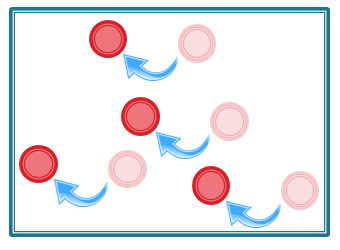
\includegraphics[width=4.7cm]{figure1_sub_a.png} \\ %TeXの基本として, \\ で緊急改行ができる.(今回の場合や行列などを除き,あまり使わない)
		\subcaption{トラジェクタ初期位置に対して一定}
		\label{subfigure:2_moving_trajector1}    
	\end{minipage}
	\begin{minipage}[t]{.3\textwidth}
		\centering
		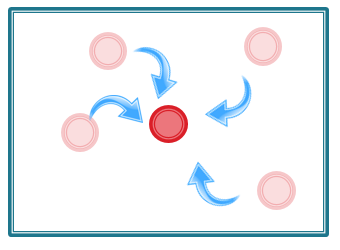
\includegraphics[width=4.7cm]{figure1_sub_b.png} \\ %TeXの基本として, \\ で緊急改行ができる.(今回の場合や行列などを除き,あまり使わない)
		\subcaption{空間上の特定の位置}
		\label{subfigure:2_moving_trajector2}
	\end{minipage}
	\begin{minipage}[t]{.3\textwidth}
		\centering
		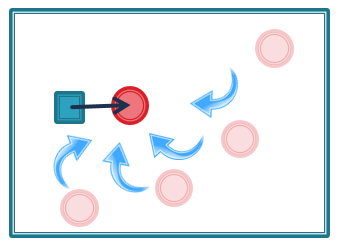
\includegraphics[width=4.7cm]{figure1_sub_c.png} \\ %TeXの基本として, \\ で緊急改行ができる.(今回の場合や行列などを除き,あまり使わない)
		\subcaption{他物体の位置に応じて変化}
		\label{subfigure:2_moving_trajector3}
	\end{minipage}
	\caption{トラジェクタ遷移の違い}
	\label{figure:2_moving_trajector}
\end{figure}
%%%%%%%%%%%%%%%%%%%%%%%%%%%%%%%%%%%%%%%%%%%%%%%%%%%%%%%%%%%%%%%%%%%%%%%%%%%%%%%%%%%%%%%%%%%%%%%%%%%%%%%
Fig.\ref{subfigure:2_moving_trajector1}はトラジェクタの初期位置を,Fig.\ref{subfigure:2_moving_trajector2}は画面中央を参照点に含めることで,Fig.\ref{subfigure:2_moving_trajector3}の特殊な事例として実現できるため,全ての物体移動動作は参照点との相対位置を考慮した目標位置を持つとしている.

このような理由から,従来研究では$L$を各物体の位置,トラジェクタの動作開始点,画面中央に定めている.

\subsection{変位}

特定の参照点に対し,変位の違いによって動作はさらに以下の2種類が存在すると定義されている.

	\begin{enumerate}
		\item 参照点を原点とし,常に一定の相対位置に遷移する
		\item 参照点を原点とし,トラジェクタの初期位置に応じて遷移先が変化する
	\end{enumerate}
これら2種類の違いについてFig.\ref{figure:2_difference_displacement}で示す.
%%%%%%%%%%%%%%%%%%%%%%%%%%%%%%%%%%%%%%%%%%%%%%%%%%%%%%%%%%%%%%%%%%%%%%%%%%%%%%%%%%%%%%%%%%%%%%%%%%%%%%%
\begin{figure}[h]
	\centering
	\begin{minipage}[t]{.4\textwidth}
		\centering
		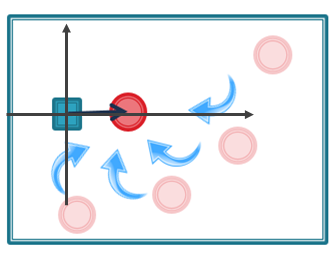
\includegraphics[width=6cm]{figure2_2_sub_a.png} \\ %TeXの基本として, \\ で緊急改行ができる.(今回の場合や行列などを除き,あまり使わない)
		\subcaption{一定の相対位置}
		\label{subfigure:2_difference_displacement1}    
	\end{minipage}
	\begin{minipage}[t]{.4\textwidth}
		\centering
		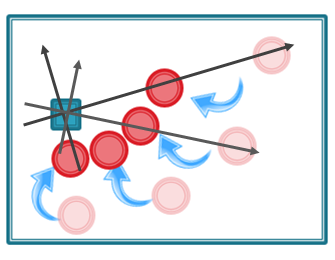
\includegraphics[width=6cm]{figure2_2_sub_b.png} \\ %TeXの基本として, \\ で緊急改行ができる.(今回の場合や行列などを除き,あまり使わない)
		\subcaption{トラジェクタの初期位置に応じて変化}
		\label{subfigure:2_difference_displacement2}
	\end{minipage}
	\caption{参照点に対する遷移の違い}
	\label{figure:2_difference_displacement}
\end{figure}
%%%%%%%%%%%%%%%%%%%%%%%%%%%%%%%%%%%%%%%%%%%%%%%%%%%%%%%%%%%%%%%%%%%%%%%%%%%%%%%%%%%%%%%%%%%%%%%%%%%%%%%
Fig.\ref{subfigure:2_difference_displacement1}は例えばトラジェクタを物体の右隣に動かすという動作などで,参照点である物体に関して常に相対位置が一定である.Fig.\ref{subfigure:2_difference_displacement2}はトラジェクタを物体に近づけるという動作などで,これは参照点となる物体とトラジェクタの初期位置の位置関係によって,参照点からの目標位置の相対位置が変化する.

従来手法ではこれらを判別する変位$k$としてそれぞれに異なる座標系を対応させている.例えばFig.\ref{subfigure:2_difference_displacement1}の動作では,参照点を原点として画面に平行な座標系を考慮することで実現することができ,Fig.\ref{subfigure:2_difference_displacement2}の動作では,参照点を原点としてトラジェクタの動作開始点に軸を向けた座標系を考慮することで実現することができる.

以下,本研究では変位$k$は座標系によって表されるとし,$Fig.\ref{subfigure:2_difference_displacement1}$のような画面空間に平行な座標系を恒等座標$k_{id}$,Fig.\ref{subfigure:2_difference_displacement2}のような,トラジェクタの動作開始点に向けた軸を持った座標系をランドマーク-トラジェクタ座標$k_{lt}$と定義する.

\subsection{学習,再現}

従来手法では教示動作が与えられたとき,以下の式を用いて尤度が最大となる参照点$\hat{l}$,座標系$\hat{k}$,隠れマルコフモデルのパラメータ$\hat{λ}$を最尤推定により学習している.
\begin{equation}
	\label{equation:sugiura}
	(\hat{λ} , \hat{k} , \hat{l}) = \mathop{\arg\max}_{λ , k , l}\sum_{i=1}^{N}\log P(F(Y_{i} , k , l_{i}) ; λ)
\end{equation}
ここで,$Y_{i}$はトラジェクタの位置,速度,加速度の時系列データ,$l_{i}$は参照点,$F(Y , k , l)$は座標系$k$,参照点$l$としたときのトラジェクタの動作軌道,$P(F,λ)$は動作軌道$F$がパラメータ$λ$の確率モデルから生成される確率である.杉浦らの研究では動作軌道を再現することを目標の一つとしていたため,確率モデルに時系列データを扱える隠れマルコフモデルを使用している.動作再現は\ref{equation:sugiura}式の最尤推定によって推定されたパラメータ$λ$を持つ隠れマルコフモデルからトラジェクタ遷移情報の時系列を生成することで実現する.
